
\chapter{Diagramas de Bode}

    Dado el siguiente sistema:

    \begin{figure}
        \centering
        \resizebox{0.6\textwidth}{!}{
            \tikzstyle{input} = [coordinate]
            \tikzstyle{output} = [coordinate]
            \tikzstyle{block} = [draw, rectangle, minimum height=3em, minimum width=4em]
            \tikzstyle{sum} = [draw, circle]
            \tikzstyle{init} = [pin edge={to-, thin, black}]

            \begin{tikzpicture}[auto, node distance=2cm, >=latex']
                \node [input, name=entrada] {};
                \node [block, right of=entrada] (planta) {$G(s)$};
                \node [output, right of=planta] (salida) {};

                \draw [->] (entrada) -- node[name=u] {$x(s)$} (planta);
                \draw [->] (planta) -- node[name=y] {$y(s)$} (salida);
            \end{tikzpicture}}
    \end{figure}

    con $G(s)$ Hurwitz estable:

    \begin{equation*}
        y(s) = G(s) x(s)
    \end{equation*}

    asumimos que la entrada es de la forma:

    \begin{equation*}
        x(s) = X \left( \frac{\omega}{s^2 + \omega^2} \right)
    \end{equation*}

    y la planta es de la forma:

    \begin{equation*}
        G(s) = \frac{p(s)}{q(s)} = \frac{p(s)}{(s + s_1) (s + s_2) \dots (s + s_n)}
    \end{equation*}

    de donde se asumen polos simples de primero orden, aunque los reslutados por obtener se mantienen si los polos no lo son.

    Al sustituir pues en la ecuación del sistema, tendremos:

    \begin{eqnarray*}
        y(s) & = & X \left( \frac{\omega}{s^2 + \omega^2} \right) \frac{p(s)}{(s + s_1) (s + s_2) \dots (s + s_n)} \\
        & = & \frac{a}{s + j \omega} + \frac{\bar{a}}{s - j \omega} + \frac{b_1}{s + s_1} + \dots + \frac{b_n}{s + s_n}
    \end{eqnarray*}

    lo cual podemos resolver obteniendo la transformada inversa de Laplace:

    \begin{equation*}
        y(t) = a e^{-j \omega t} + \bar{a} e^{j \omega t} + b_1 e^{-s_1 t} + \dots + b_n e^{-s_n t}
    \end{equation*}

    lo cual implica que tendremos una salida en estado estacionario:

    \begin{equation*}
        y_{ss}(t) = \lim_{t \to \infty} y(t) = a e^{-j \omega t} + \bar{a} e ^{j \omega t}
    \end{equation*}

    es decir, cuando $t$ tiende a $infty$ todos los polos del sistema se eliminan y nos queda el comportamiento de la entrada a seguir.

    Por otro lado, para obtener los valores de $a$ y $\bar{a}$ aplicamos fracciones parciales y obtenemos:

    \begin{eqnarray*}
        a & = & \left. G(s) X \left( \frac{\omega}{s^2 + \omega^2} \right) + (s + j \omega) \right|_{s=-j \omega} = - G(-j \omega) X \frac{1}{2j} \\
        \bar{a} & = & \left. G(s) X \left( \frac{\omega}{s^2 + \omega^2} \right) + (s - j \omega) \right|_{s=j \omega} = G(j \omega) X \frac{1}{2j}
    \end{eqnarray*}

    de donde sabemos que $G(j \omega)$ lo podemos escribir como su magnitud multiplicado por una exponencial de mangitud unitaria con el angulo deseado:

    \begin{eqnarray*}
        G(j \omega) & = & \left| G(j \omega) \right| e^{j \phi} \\
        G(-j \omega) & = & \left| G(j \omega) \right| e^{-j \phi}
    \end{eqnarray*}

    en donde $\phi = \phase{G(j \omega)} = \arctan{\left( \frac{\Im{G}}{\Re{G}} \right)}$.

    Por lo tanto, $a$ y $\bar{a}$ los podemos escribir como:

    \begin{eqnarray*}
        a & = & - \left| G(j \omega) \right| e^{-j \phi} X \frac{1}{2j} \\
        \bar{a} & = & \left| G(j \omega) \right| e^{j \phi} X \frac{1}{2j}
    \end{eqnarray*}

    Tomando esto en cuenta, la salida en estado estacionario nos quedará:

    \begin{eqnarray*}
        y_{ss}(t) & = & X \left| G(j \omega) \right| \frac{e^{j(\omega t + \phi)} - e^{-j(\omega t + \phi)}}{2j} \\
        & = & X \left| G(j \omega) \right| \sin{(\omega t + \phi)} \\
        & = & y \sin{(\omega t + \phi)}
    \end{eqnarray*}

    en donde $y = X \left| G(j \omega) \right|$ y $\phi = \phase{G(j \omega)}$.

    \newpage
    \section{Factores de primer orden}
        Para analizar ahora el comportamiento de una planta con factores de primer orden, proponemos el sistema siguiente:

        \begin{equation*}
            G(s) = \frac{1}{Ts + 1}
        \end{equation*}

        el cual tiene magnitud y fase:

        \begin{eqnarray*}
            \left| G(j \omega) \right| & = & \left| \frac{1}{j \omega T + 1} \right| = \frac{1}{\sqrt{1 + (\omega T)^2}} \\
            \left| G(j \omega) \right|_{dB} & = & 20 \log{\left| G(j \omega) \right|} = -20 \log{\sqrt{1 + (\omega T)^2}} \\
            \phi & = & - \arctan{(\omega T)}
        \end{eqnarray*}

        en donde a la magnitud le hemos sacado el $log_{10}$ y multiplicado por $20$ para expresarla en $dB$.

        De estas expresiones podemos ver, que para diferentes valores de $\omega T$ obtendremos diferentes valores de magnitud:

        \begin{eqnarray*}
            \omega T \ll 1 & \implies & \left| G(j \omega) \right|_{dB} \approx -20 \log{\sqrt{1}} = 0 dB \\
            \omega T \gg 1 & \implies & \left| G(j \omega) \right|_{dB} \approx -20 \log{\sqrt{(\omega T)^2}} = -20 \log{(\omega T)} dB \\
            \omega T = 1 & \implies & \left| G(j \omega) \right|_{dB} = -20 \log{\sqrt{2}} \approx -3 dB
        \end{eqnarray*}

        y de fase:

        \begin{eqnarray*}
            \omega T \ll 1 & \implies & -\arctan{(\omega T)} \approx - \arctan{0} = 0^o \\
            \omega T \gg 1 & \implies & -\arctan{(\omega T)} \approx - \arctan{\infty} = -90^o \\
            \omega T = 1 & \implies & -\arctan{(\omega T)} = - \arctan{1} = -45^o
        \end{eqnarray*}

        Con estas expresiones podemos trazar asintotas las cuales nos ayudarán a gráficar el diagrama de Bode de la figura~\ref{fig:bodeprimerorden}.

        \begin{figure*}
            \centering
            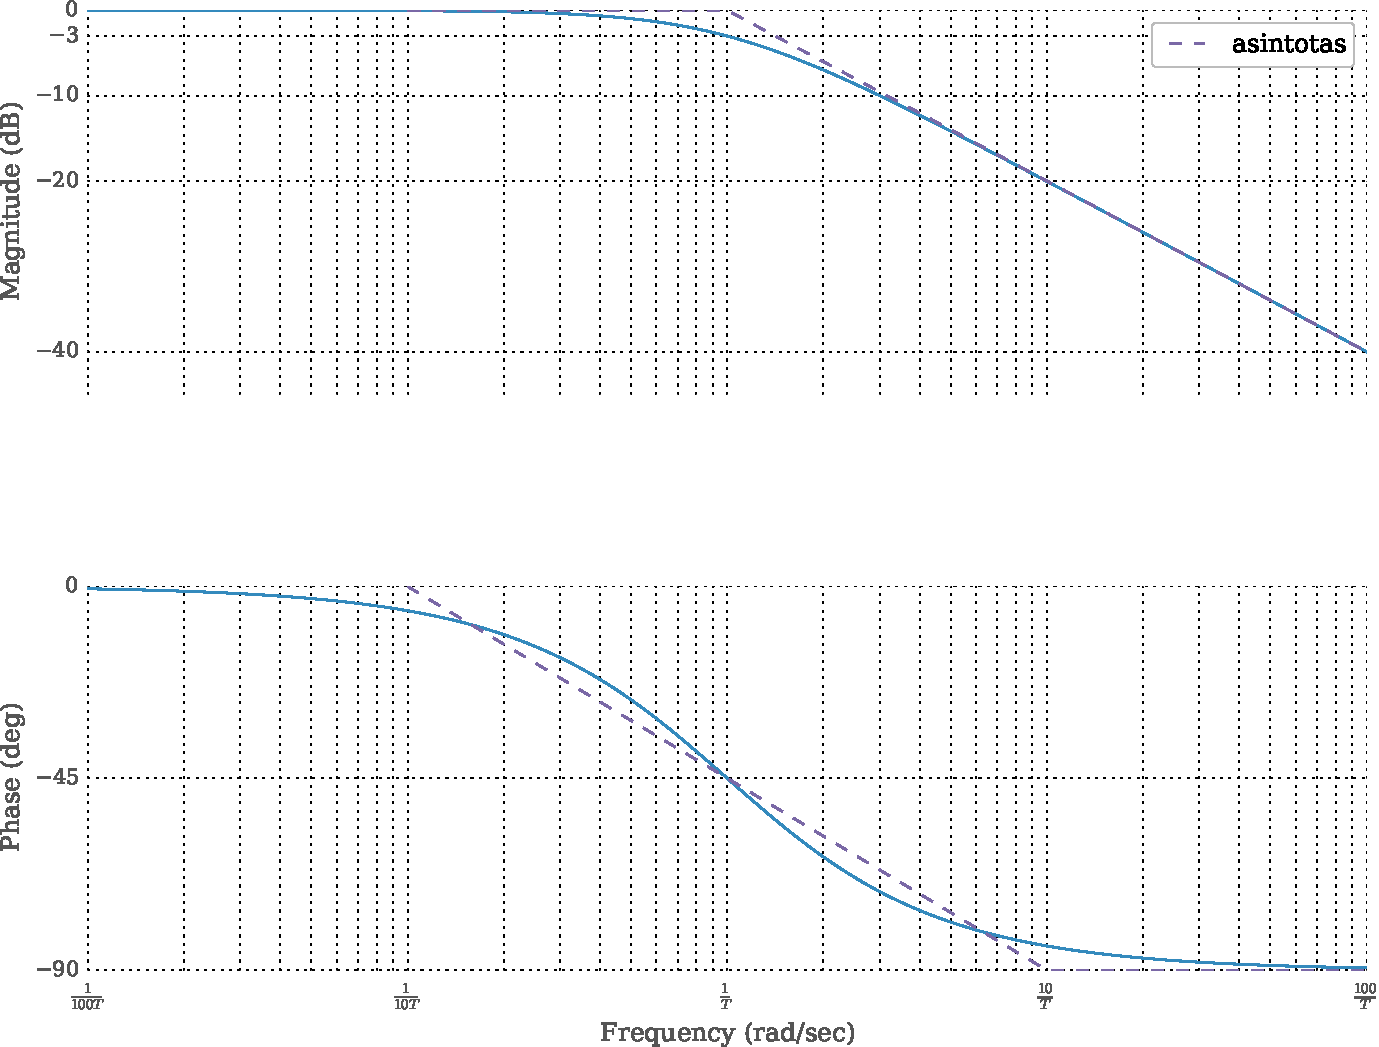
\includegraphics[width=0.9\textwidth]{./imagenes/bodeprimerorden.pdf}
            \caption{\label{fig:bodeprimerorden}Diagrama de Bode de sistema de primer orden.}
        \end{figure*}

    \section{Factor integral}
        \faltante{Falta escribir apunte}
    \section{Factor derivativo}
        \faltante{Falta escribir apunte}
    \section{Factores de segundo orden}
        \faltante{Falta escribir apunte}
    \section{Frecuencia de resonancia $\omega_n$ y valor par de resonancia $M_R$}
        \faltante{Falta escribir apunte}
